\documentclass{jot}
% Use the documentclass option 'lineno' to view line numbers

% Enter the JOT metadata in the following 
\usepackage{multirow}

\jotdetails{
    volume=vv,      % volume
    number=nn,       % number or issue
    articleno=aa,   % article number, eg a1 for research articles, e for editorials
    year=2022,      % year
    license=ccby    % choose from ccby, ccbynd, ccbyncnd
}
\newcommand{\command}[1]{{\color{codepurple}\texttt{\textbackslash #1}}}
\newcommand{\param}[1]{{\color{blue}\texttt{#1}}}
% Select the article type
\articletype{regular} 
    % {editorial} editorial 
    % {regular} regular contribution
    % {manual} manual
    % {column} column

\title{Towards behavioral consistency in multi-modeling}

\author[$\ast$]{Tim Kräuter}
% Arbitrary co-author order. Everyone contributed significantly.
\author[$\ast\dagger$]{Harald König}
\author[$\ast$]{Adrian Rutle}
\author[$\ast$]{Yngve Lamo}
\author[$\ddagger$]{Patrick Stünkel}

\affil[$\ast$]{Western Norway University of Applied Sciences, Bergen, Norway}
\affil[$\dagger$]{University of Applied Sciences, FHDW, Hannover, Germany}
\affil[$\ddagger$]{Haukeland Universitetssykehus, Bergen, Norway}

\keywords{	
Global behavioral consistency,
Consistency verification,
Multi-modeling,
Heterogeneous models,
Rewriting Logic,
Graph transformation
}

\runningtitle{Towards behavioral consistency in multi-modeling} % For use in the internal pages 

\runningauthor{Kräuter \textit{et al.}}

\usepackage{amsthm} % for proofs
\usepackage{amsmath} % theorems, definitions, etc.
\newtheorem{definition}{Definition}
\newcommand{\definitionautorefname}{Definition}

% Table

\usepackage{glossaries}
\usepackage{cleveref} % Reference footnotes.
\crefformat{footnote}{#2\footnotemark[#1]#3}

\newacronym{ltl}{LTL}{Linear temporal logic}
\newacronym{mde}{MDE}{Model-driven engineering}
\newacronym{bpmn}{BPMN}{Business Process Modeling Notation}
\newacronym{uml}{UML}{Unified Modeling Language}
\newacronym{csp}{CSP}{Communication Sequential Processes}
\newacronym{ccsl}{CCSL}{Clock Constraint Specification Language}
\newacronym{dsl}{DSL}{Domain-specific language}

% correct bad hyphenation here
\hyphenation{be-ha-vi-o-ral}

% Listing settings

\lstdefinelanguage{Interaction}[]{Java}{
    morekeywords={synchronize},
    comment=[l]{---},
}

\lstset{emph={  
    rl
    },emphstyle={\color{blue}\bfseries}
}

\begin{abstract}
%ABOUT: Introduce multi-model and motivate global behavior checking
Multiple interacting systems are needed to realize the requirements of complex domains.
Describing the interactions between these systems and checking their global behavioral consistency is a general, well-known challenge in software engineering.
To address this challenge, model-driven software engineering utilizes abstract representations of the constituting systems and their interactions, resulting in a \emph{multi-model} representing the overall software.
In such a multi-modeling setting, global consistency rules must be satisfied by a set of heterogeneously typed models to guarantee a desired \emph{global behavior}.
In this paper, we propose a novel approach for behavioral consistency management of heterogeneous multi-models.
The approach introduces a workflow in which we
(i) align the individual models and specify their \emph{interactions}, 
(ii) generate a \emph{global execution semantics} for the multi-model, and finally,
(iii) define and check \emph{global properties} which should be satisfied by the multi-model.
Our approach is independent of a particular formalism as an underlying global execution semantics, and the current two implementations utilize rewriting logic (Maude) and graph transformations (Groove), respectively.
\end{abstract}

% TODO: Comment in after acceptance and helpful feedback.
% \acknowledgment{We want to thank the anonymous reviewers for their valuable comments and helpful suggestions.}

\begin{document}    
\maketitle
\urlstyle{rm}

\section{Introduction} \label{sec:introduction}
% Introduce multi-model
\gls*{mde} addresses the increasing complexity of software systems by employing models to describe the different aspects of the system.
In this way, \gls*{mde} promotes a clear separation of concerns and raises the abstraction level throughout the entire development process \cite{franceModeldrivenDevelopmentComplex2007}.
These models are then used to generate portions of the system leading to an increase in productivity and reduction of errors \cite{brambillaModeldrivenSoftwareEngineering2017}.
As multiple interacting systems are needed to realize the requirements of complex domains, a set of corresponding models would be needed to represent these systems and their interactions.
Such a collection of inter-related models is referred to as a \emph{multi-model} \cite{boronatWhatMultimodelingLanguage2009, stunkelComprehensiveSystemsFormal2021}, which is usually heterogeneous, meaning it consists of models conforming to different modeling languages.
% Consistency in multi-modeling
Models in a multi-model contradicting each other can lead to problems during development, system generation, and system execution.
Consequently, continuous multi-model consistency management during the development process is a significant issue for multi-models \cite{spanoudakisInconsistencyManagementSoftware2001, cicchettiMultiviewApproachesSoftware2019}.

% Consistency can be checked for a set of structural models
Recent research describes methods to check the structural consistency of a multi-model \cite{stunkelComprehensiveSystemsFormal2021, klareCommonalitiesPreservingConsistency2019}.
Structural models, like UML class diagrams, describe structural aspects of systems, i.e., domain concepts and relations between these concepts.
This is usually referred to as the static semantics of the software system as it only describes the set of valid instances or states of the system.
% Challenge: Consistency for a set of behavioral models.
Nevertheless, approaches to multi-model consistency management must also include a means to maintain \emph{behavioral consistency} since behavioral models, like \gls*{bpmn} models, are associated with execution semantics describing dynamic aspects of the system \cite{objectmanagementgroupUnifiedModelingLanguage2017, objectmanagementgroupBusinessProcessModel2013}.

% Existing solutions. But they are not sufficient!
Several approaches exist for checking the consistency of pairs of behavioral models.
For example, consistency checking for sequence diagrams and statecharts was implemented using Petri nets \cite{yaoConsistencyCheckingUML2006} and \gls*{csp} \cite{kusterExplicitBehavioralConsistency2003}.
Moreover, some approaches for model simulation in heterogeneous scenarios have been developed, such as Ptolemy \cite{ekerTamingHeterogeneityPtolemy2003, leeDisciplinedHeterogeneousModeling2010} and GEMOC studio \cite{deantoniModelingBehavioralSemantics2016, varalarsenBCoolBehavioralCoordination2016}.
However, current approaches either only allow for consistency checking of two behavioral models or do not allow for definition and checking of global behavioral properties.

% Our approach summarized.
We propose a novel approach for consistency management of heterogeneous multi-models, which allows us to define and check \emph{global} behavioral properties.
Our approach facilitates specifying \emph{interactions} between potentially heterogeneous behavioral models, which are in turn used to generate global execution semantics.
Although our approach is independent of a particular formalism as an underlying global execution semantics, the current implementations utilize the rewriting logic tool Maude and the graph transformation tool set Groove (see \autoref{sec:maude_execution_semantics}).
The generation of global execution semantics is \textit{fully automatic} and results in term rewriting rules/graph transformation rules usable by Maude/Groove for the global system.
Afterward, we can use the built-in verification mechanisms in Maude/Groove to check the previously defined global behavioral properties.
A potential future advantage of Maude is that it additionally supports the verification of Real-Time systems \cite{olveczkySemanticsPragmaticsRealTime2007, duranVerifyingTimedBPMN2017}, which is useful when models with time aspects have to be analyzed in the future.

% Paper outline
The remainder of this paper is structured as follows.
We introduce a simplified use case (\autoref{sec:usecase}) before explaining our behavioral consistency management approach in detail (\autoref{sec:behavioral_consistency_checking}).
Afterward, we show how we can use the Groove tool set and the Maude system to check behavioral consistency (\autoref{sec:global_execution_semantics}).
Furthermore, we examine related work in \autoref{sec:related_work}.
Finally, we discuss the state space explosion problem in \autoref{sec:state_space_explosion} and conclude in \autoref{sec:conclusion_and_future_work}.

\section{Use Case} \label{sec:usecase}
This section motivates our approach by a simplified use case in which a traffic management system is developed to guide the traffic at a T-Junction with three traffic lights.
The traffic management system should control the traffic by switching between the two traffic phases highlighted in \autoref{fig:junction-phases}.
In addition, it must fulfill the following two requirements.
First, it must guarantee safe traffic by changing the three traffic lights, A, B, and C, correctly.
Second, it should prioritize arriving buses, i.e., switch the traffic lights quicker than usual to let an approaching bus pass (early green).
This so-called bus priority signal is a widely implemented technique to improve service and reduce delays in public transport.

\begin{figure}[h]
    \centering
    % warning is fine since it does not visually overflow.
    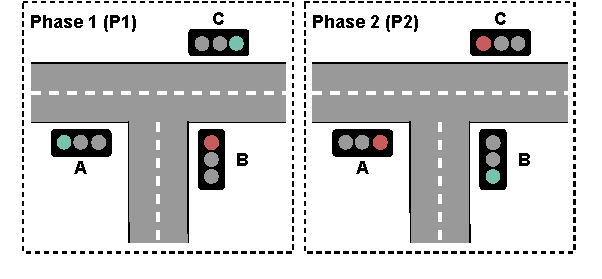
\includegraphics[width=0.5\textwidth]{figures/phases.pdf}
    \caption{Traffic phases of a T-Junction}
    \label{fig:junction-phases}
\end{figure}

To develop the behavior of the traffic management system, we follow an \gls*{mde} approach.
First, we model the behavior of a traffic light as a \gls*{uml} state machine, and then we use \gls*{bpmn} to model the different traffic phases of the T-Junction, including the prioritization of approaching buses.

Using different behavioral modeling languages in the use case has two reasons.
First, two software development teams might work on the system in parallel but prefer different modeling languages.
Second, each team is free to choose the most appropriate modeling language for defining their part of the system.
In this use case, the behavior of a traffic light and a T-Junction differs significantly in complexity and requirements, resulting in the use of two different behavioral modeling languages, namely \gls*{uml} state machines, and \gls*{bpmn}.

The behavior of a traffic light is straightforward since it uses only three colors to guide the traffic.
\autoref{fig:trafficLight} shows the typical European\footnote{Traffic lights in other parts of the world might not show red and amber simultaneously before switching to green.} traffic light that switches from \textsf{red} to \textsf{red-amber}, \textsf{green}, \textsf{amber}, and back to \textsf{red}.
The start state of the traffic light in \autoref{fig:trafficLight} is \textsf{red} but can be any of the four possible states.

\begin{figure}[h]
    \centering
    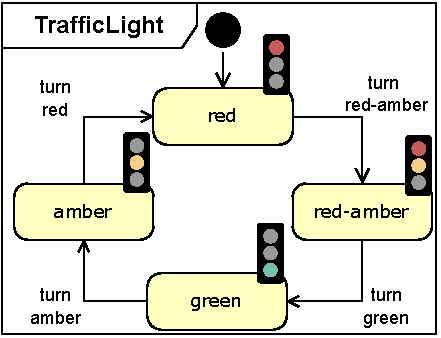
\includegraphics[width=0.35\textwidth]{figures/trafficLight.pdf}
    \caption{Traffic light state machine model}
    \label{fig:trafficLight}
\end{figure}

However, the T-Junction's behavior is more complex since it should coordinate the three traffic lights and communicate with approaching buses to implement bus priority.
Consequently, we are using \gls*{bpmn} to model this aspect of the system's behavior and utilize \gls*{bpmn} message and signal events to implement the communication with approaching buses.

We model two processes, one for the T-Junction and one for the Bus.
Each process is modeled in its own \gls*{bpmn} \emph{pool}.
A pool is depicted as a horizontal lane with a name on the left.
Message flows (arrows with dashed lines) are only allowed between two different pools.

\autoref{fig:t_junction} shows how a possible controller for a T-Junction behaves in the traffic management system\footnote{All models and their source files can be found in \cite{krauterArtifactsBehavioralConsistency2022}.\label{footnote:fullModels}}.
When a T-Junction controller is started, we assume that the traffic lights are showing the colors according to phase 1 (see \autoref{fig:junction-phases}).
Thus, the controller enters a subprocess called phase 1 (see \autoref{fig:communication} top right), which we describe together with the subprocess called phase 2 later.
However, when a fixed amount of time has passed, the subprocess is interrupted by the attached timer boundary event.
Then, the controller executes the next activity and switches to phase 2.
The controller will pass a throwing signal event before entering a subprocess for phase 2 and repeat the same steps.
This signal event represents a broadcast to all buses waiting for traffic light B to become green.
After switching back from phase 2 to phase 1 and signaling that traffic lights A and C are green, the controller can stop or execute the described steps again.
Typically, the controller does not stop, which is indicated by the default sequence flow going back to the process beginning.

% T-Junction BPMN model
\begin{figure*}[h]
    \centering
    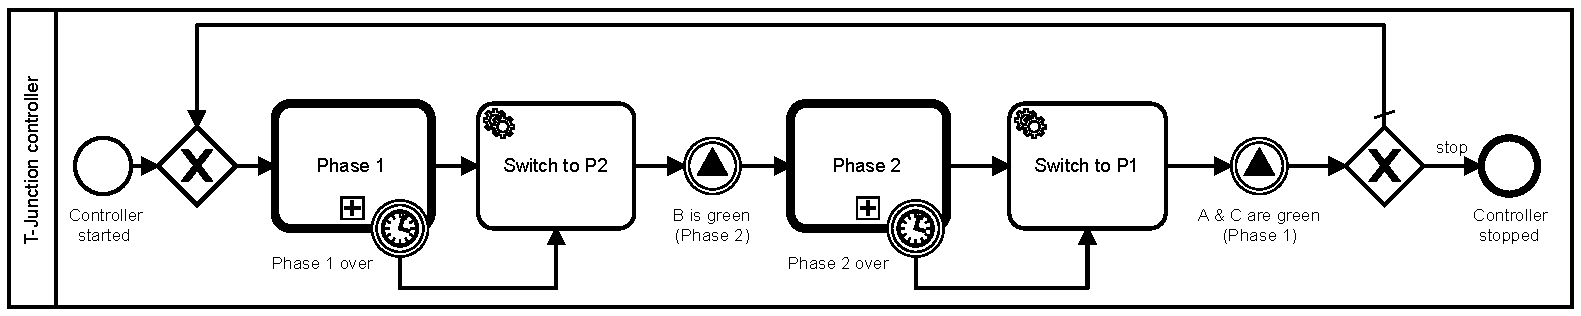
\includegraphics[width=1\textwidth]{figures/t-junction.pdf}
    \caption{Model for a T-Junction controller}
    \label{fig:t_junction}
\end{figure*}

% Bus and Phase 1 BPMN model
\begin{figure*}[ht]
    \centering
    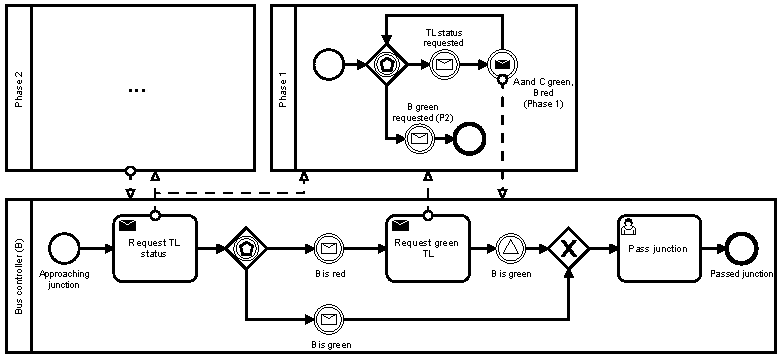
\includegraphics[width=1\textwidth]{figures/communication.pdf}
    \caption{Model for a bus with direction B and its communication with a T-Junction}
    \label{fig:communication}
\end{figure*}

\autoref{fig:communication} shows the communication of a bus with the subprocess phase 1.
The \gls*{bpmn} model and communication for phase 2 of the controller can be defined accordingly \cref{footnote:fullModels}.

The phase 1 model uses an event-based gateway to respond to two different kinds of messages.
First, the traffic light status can be requested, which is answered by sending a message declaring that the traffic lights A and C are green while B is red.
Moreover, early green for traffic light B can be requested.
This request ends the subprocess, and the controller immediately switches to phase 2 (see \autoref{fig:t_junction}), which results in the traffic light B turning green.

The bottom of \autoref{fig:communication} shows the controller for a bus parameterized with direction B.
It will first request the traffic light status to determine if traffic light B is green.
If it is green, the bus can pass the junction.
However, if it is red, the bus requests to change B to green and waits for a signal that the controller has changed the traffic light.
After receiving the signal, the bus passes the junction.
A \gls*{bpmn} model for a bus controller parameterized with the direction A or C looks nearly identical.
In addition, the bus controller also communicates with the phase 2 subprocess, which we only hint at in \autoref{fig:communication}\cref{footnote:fullModels}.
The phase 2 subprocess has the same structure as the phase 1 subprocess but reports that A and C are red, while B is green.
Similarly, it terminates if green is requested for A or C.

Having developed behavioral models for the system, we want to check the previously stated \emph{safe traffic} requirement while buses are prioritized.
We can lower the overall development cost if we find bugs related to these requirements as early as possible during system development.
However, the traffic light model is currently not related to the T-Junction and bus models, which is a problem since the T-Junction is supposed to control the traffic lights, for example, when it switches between the two traffic phases.
In addition, the system has to manage multiple slightly different instances of the behavioral models.
For example, there are three traffic lights at one T-Junction starting in different states, i.e., showing different colors and buses approaching the T-Junction from one of the three directions.
Consequently, we need a model of the system to allow us to define interactions between the models and configure instances of the behavioral models contained in the multi-model.

The resulting model called the \emph{system relationship model} is shown in \autoref{fig:systemRelationshipModel} using a class diagram-like syntax.
It contains one class for each behavioral model and associations to depict behavioral relationships, leading to possible interactions.
In addition, it contains enumerations to parameterize the behavioral models. 

\begin{figure}[h]
    \centering
    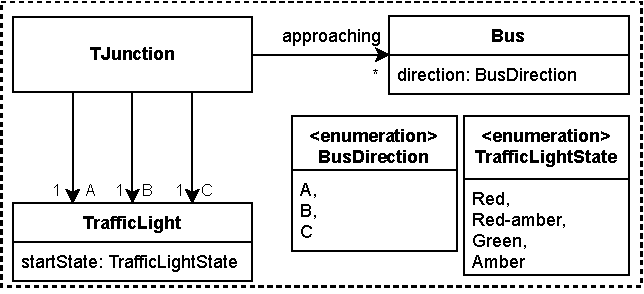
\includegraphics[width=0.45\textwidth]{figures/systemRelationShipModel.pdf}
    \caption{System relationship model of the traffic management system}
    \label{fig:systemRelationshipModel}
\end{figure}

A \textsf{TJunction} has three associated \textsf{TrafficLight}s, A, B, and C, and a set of currently approaching \textsf{Bus}es.
A \textsf{TrafficLight} has four possible \textsf{TrafficLightState}s and an attribute to define its \textsf{startState}.
A \textsf{Bus} has a \textsf{direction} that indicates which \textsf{TrafficLight} of the T-Junction it is approaching.

Finally, using the system relationship model, we can define a test configuration of our traffic management system to check its requirements.
\autoref{fig:test_config} depicts the test system configuration, an instance of the system relationship model.
First, it contains three instances of the traffic light behavioral model, representing the three traffic lights, \textbf{A}, \textbf{B}, and \textbf{C}.
Second, it contains an instance of the T-Junction behavioral model, which is connected to the three traffic lights, and two instances of the bus behavioral model.
Thus, the test system configuration describes a system that controls one T-Junction with three traffic lights and two buses approaching from directions A and C.

\begin{figure}[h]
    \centering
    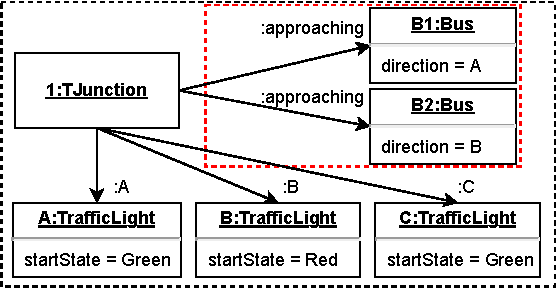
\includegraphics[width=0.45\textwidth]{figures/test_config.pdf}
    \caption{Test system configuration}
    \label{fig:test_config}
\end{figure}

First, we would like to check the safe traffic requirement.
Since we only want to check system conformance concerning the two traffic phases, we do not need to include the two buses depicted in the red dotted square in \autoref{fig:test_config} in the analysis.
We cannot simply assert that the system is either in phase 1 or phase 2 since there are intermediate states during the transition between the two phases, which are allowed.
By consulting \autoref{fig:trafficLight}, we can, for example, expect a state in which traffic lights A and C are amber, and traffic light B is red-amber before reaching phase 2.
However, we can define \emph{safe traffic} as the absence of \emph{unsafe traffic}, which is easier to define.

For the T-Junction, unsafe traffic occurs if traffic light A is green or amber and traffic light B is green or amber simultaneously.
In addition, the same state combinations are forbidden for traffic lights B and C.
Unsafe traffic occurs only in these situations since green/amber means that cars are allowed to pass, while red/red-amber means cars are not/not yet allowed to pass.
We can formalize the consistency requirements as safety properties in \gls*{ltl}, i.e., states that should never be reached.
The resulting global properties \ref{eq:property1} and \ref{eq:property2} are the following\footnote{We assume the existence of atomic propositions for each traffic light state. 
The propositions are formalized later.}:

\begin{align}
    \square\neg((A_{green} \lor A_{amber}) \land (B_{green} \lor B_{amber})) \label{eq:property1} \\
    \square\neg((C_{green} \lor C_{amber}) \land (B_{green} \lor B_{amber})) \label{eq:property2}
\end{align}

If we include buses \textsf{B1} and \textsf{B2} in the system, we would like to check that they cannot pass when their traffic light is red or red-amber.
Concretely, this means the \textsf{Pass Junction} activity should not execute while the corresponding traffic light is \textsf{red} or \textsf{red-amber}.
We formalize these requirements again by using \gls*{ltl} safety properties \ref{eq:property3} and \ref{eq:property4}\footnote{The atomic proposition $B1_{passing}\, / \,B2_{passing}$ represents that \textsf{Pass Junction} (see \autoref{fig:communication}) has started but not finished yet, i.e., there is a token in the activity when using \gls*{bpmn} token semantics \cite{objectmanagementgroupBusinessProcessModel2013}.}.

\begin{align}
    \square\neg(B1_{passing} & \land (A_{red} \lor A_{red-amber})) \label{eq:property3} \\
    \square\neg(B2_{passing} & \land (B_{red} \lor B_{red-amber})) \label{eq:property4}
\end{align}

However, to check the global properties, we must execute the system with the behavior specified in the behavioral models according to the test configuration.
This is not straightforward since the multi-model of the use case consists of a system relationship model relating two heterogeneous behavioral models.
In addition, the system configuration instantiates two of the behavioral models multiple times with different parameters.
Furthermore, we face the problem that the models are not independent of each other.
For example, the T-Junction controller must control when the traffic lights A, B, and C switch their states.
Thus, if we were to run the models independently in parallel, the properties would be violated.

Current approaches can only simulate a set of interacting heterogeneous behavioral models, as discussed in \autoref{sec:introduction}.
However, they do not allow multiple instances of a behavioral model (without duplicating it) nor provide concrete means to define and check \emph{global} behavioral properties.
Thus, they are not capable of checking multi-model behavioral consistency.
A multi-model is behaviorally consistent if it satisfies all of its behavioral properties.
A behavioral property is given in temporal logic, for example, \gls*{ltl} in the use case, and is characterized as \emph{local} if it constrains only one model and as \emph{global} if it spans two or more models in a multi-model.
Furthermore, global properties are dependent on the system configuration, i.e., the instance of the system relationship model used.
In the remainder of this paper, we will describe our approach to address behavioral consistency in multi-modeling and apply it to this use case.

\section{Behavioral consistency management} \label{sec:behavioral_consistency_checking}
% Introduce the overall approach using the workflow somehow here and follow it.
\autoref{fig:approach} depicts our approach to behavioral consistency management using a \gls*{bpmn} diagram.
We leave potential consistency restoration as a problem for future work.

\begin{figure}[h]
    \centering
    % https://cawemo.com/share/a531b027-0475-4050-8b7c-9de631abbe13
    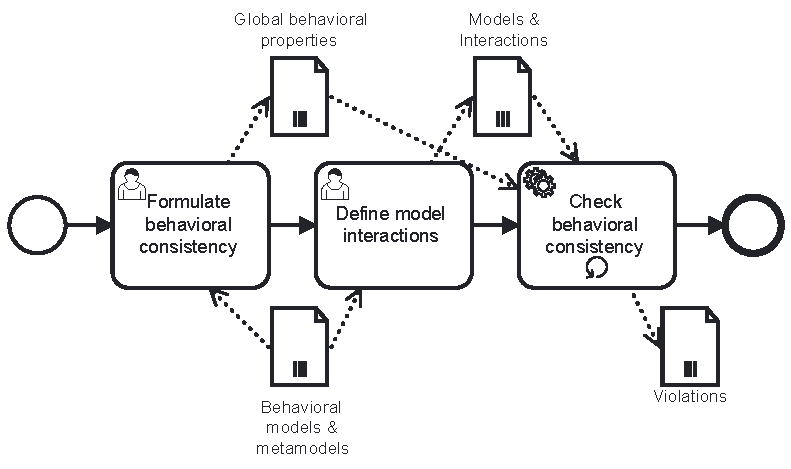
\includegraphics[width=0.475\textwidth]{figures/workflow.pdf}
    \caption{Behavioral consistency management workflow}
    \label{fig:approach}
\end{figure}

Our approach can be summarized in three steps.
First, we formulate the behavioral consistency requirement in terms of global behavioral properties for the given behavioral models.
This step also leads to a system relationship model, describing which behavioral models can interact.
Second, we define interactions between the behavioral models based on the system relationship model.
Based on these interactions and the behavioral models, we automatically generate execution semantics for the global system.
Finally, given a system configuration and consistency requirements, we can check these requirements using the generated global execution semantics.
Consistency checking potentially leads to violations, describing counter-examples of how the global behavioral properties can be invalidated.

We will now describe our approach in detail by first explaining the \textit{system relationship model} concept and then the three steps in the workflow.

\subsection{System relationship model}
We assume a set of behavioral models describing the system, where each model must conform to a metamodel.
A metamodel can be defined by a class diagram/grammar for graphical/textual modeling languages.
The metamodel ensures that the corresponding models are machine-readable, which is crucial when automating parts of the consistency checking.
In addition, some of the behavioral models \emph{interact} to realize the global system behavior.
A system relationship model describes which behavioral models exist in the system and how they are related.
The system relationship \emph{metamodel} is depicted in \autoref{fig:systemRelationshipMetamodel}.

\begin{figure}[h]
    \centering
    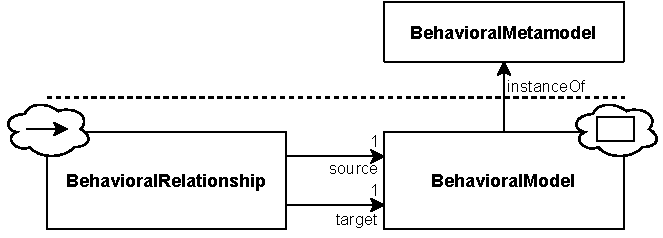
\includegraphics[width=0.45\textwidth]{figures/systemRelationshipMetamodel.pdf}
    \caption{System relationship metamodel \\ (without attributes and enumerations)}
    \label{fig:systemRelationshipMetamodel}
\end{figure}
% Also: Behavioral relationships have multiplicities to restrict possible system configurations. But already known for structural models and thus not really relevant here.

Behavioral models typed in \textsf{BehavioralMetamodel}s can be connected by \textsf{BehavioralRelationship}s to allow for interactions.
We are using a \gls*{uml} class diagram-like syntax to define system relationship models, where each class corresponds to a behavioral model (typed in a \textsf{BehavioralMetamodel}), while each association corresponds to a \textsf{BehavioralRelationship} (see concrete syntax depicted in clouds).
Thus, a system relationship model does \emph{not} describe the structure of a system, but rather behavioral relationships between the behavioral models of a system.
The behavioral relationships will be crucial to define interactions between the models in the first step of our approach.

In addition, we allow enumerations and their use as attributes for behavioral models in the system relationship model.
This prevents duplication of behavioral models because we can use the attributes as parameters, for example, to define the start state in a state machine (see \autoref{fig:systemRelationshipModel}).
Different instances of the system relationship model can be used to analyze the global behavior of \emph{different} system configurations by changing the attribute values and behavioral model instances.

The use case utilizes state machine and \gls*{bpmn} models.
Thus, according to \autoref{fig:systemRelationshipMetamodel} there must be a metamodel for state machines and \gls*{bpmn} process models.
\autoref{fig:fsm_metamodel} shows the metamodel for finite state machines (ignore the purple coloring for now).
It is defined by a \gls*{uml} class diagram with additional information depicted in clouds.
The clouds define a concrete syntax for state machines inspired by \gls*{uml} statecharts.
A model in this concrete syntax, such as the traffic light model (see \autoref{fig:trafficLight}), can automatically be translated to abstract syntax and typed in the metamodel.

% state machine
\begin{figure}[h]
    \centering
    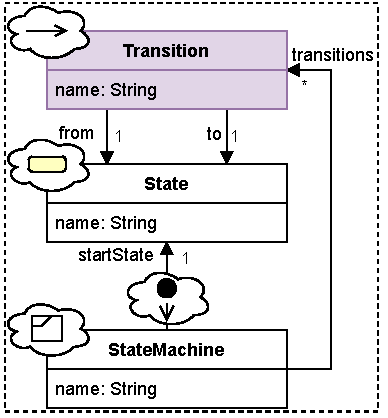
\includegraphics[width=0.275\textwidth]{figures/state_machine_metamodel.pdf}
    \caption{Finite state machine metamodel $M^1$}
    \label{fig:fsm_metamodel}
\end{figure}

A \textsf{StateMachine} has a \textsf{startState} and \textsf{transitions}, whereas each \textsf{Transition} connects two \textsf{State}s.
The states of a state machine are not explicitly modeled but can be derived from the states connected by the transitions of a state machine, assuming no isolated states.

Similarly, we must define a metamodel for \gls*{bpmn} process models.
\autoref{fig:bpmn_metamodel} shows a simplified metamodel for \gls*{bpmn} (ignore the purple coloring for now).
Once more, we have attached concrete syntax elements.

% bpmn (subset of the needed constructs)
\begin{figure}[h]
    \centering
    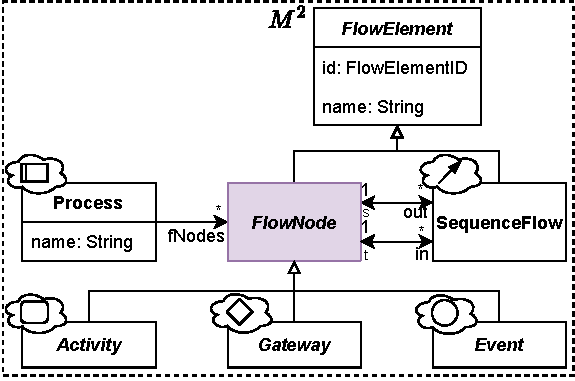
\includegraphics[width=0.475\textwidth]{figures/bpmn_metamodel.pdf}
    \caption{Simplified BPMN metamodel $M^2$ \cite{objectmanagementgroupBusinessProcessModel2013}}
    \label{fig:bpmn_metamodel}
\end{figure}

A \gls*{bpmn} \textsf{Process} contains a set of \textsf{FlowNode}s connected by \textsf{SequenceFlow}s.
A \textsf{FlowNode} can be an \textsf{Activity}, \textsf{Gateway}, or \textsf{Event}.
Concrete activities, gateways and events are defined in the full \gls*{bpmn} metamodel \cite{objectmanagementgroupBusinessProcessModel2013}. % See BPMN class diagrams in figures 10.104/10.6/10.69.

\subsection{Formulate behavioral consistency}
% Create a system relationship model (driven by the atomic properties and potential interactions).
The \textbf{first step} to formulate behavioral consistency is to create a system relationship model for the given multi-model.
Typically, each behavior model in the multi-model is represented in the system relationship model, depicted as a box (see \autoref{fig:systemRelationshipMetamodel}).
In addition, one has to add behavioral relationships between the behavioral models.
To find out which behavioral relationships exist, one should look at the desired interactions of the behaviors in the multi-model and the desired global behavioral properties.

First, interactions in the second step of the workflow can only be defined if there exists a behavioral relationship between the interacting behaviors.
Second, if a global property applies to two behavioral models, there should be a direct or indirect behavioral relationship between the models.
Otherwise, the global property could be divided into two local properties, which could be checked independently on the two behavioral models.

For example, the system relationship model for the use case (see \autoref{fig:systemRelationshipModel}) has three behavioral relationships from \textsf{TJunction} to \textsf{TrafficLight} since a T-Junction controller interacts with three different traffic lights A, B, and C.
Furthermore, there is a behavioral relationship from \textsf{TJunction} to \textsf{Bus} because we want to check the safety properties \ref{eq:property3} and \ref{eq:property4}. 

% Properties describe snapshots of systems. Thus, we need additional models. The snapshot metamodels.
The \textbf{second step} to formulate behavioral consistency is to define the global behavioral properties.
These properties are defined using temporal logic, for example, \gls*{ltl} in the use case.
Temporal logic properties are built upon a set of atomic propositions which are either true or false in a given state.
However, there is currently no model describing how a state/\emph{snapshot} of a behavioral model is represented during execution.
Consequently, we introduce a new model type called the \emph{snapshot metamodel}, which defines the structure of a state for a given formalism.
There must be one snapshot metamodel for each formalism used in the multi-model.
Generally, we assume that the states of behavioral models can be modeled as a class diagram.
Thus, snapshot metamodels are defined using class diagrams, and each state is a set of objects conforming to the corresponding snapshot metamodel.
Furthermore, the transitions between those states depend on the given behavioral models and their semantics.

For example, in the use case, we define a snapshot metamodel for state machines and \gls*{bpmn}.
The snapshot metamodel for a state machine is straightforward since a state machine can only be in one state at a time, as shown in \autoref{fig:fsm_snapshot_model}.
Since we are only interested in the current state and not the history of states, we call this a \emph{state machine snapshot}.
We are reusing the concrete syntax elements from the metamodel level.
In addition, each snapshot metamodel has a root element in our approach, highlighted in light blue in \autoref{fig:fsm_snapshot_model}.
\begin{figure}[h]
    \centering
    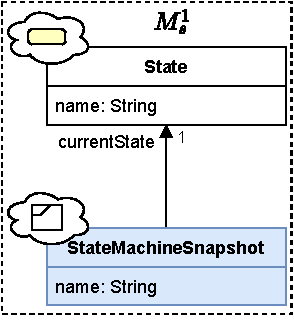
\includegraphics[width=0.22\textwidth]{figures/state_machine_s_model.pdf}
    \caption{Finite state machine snapshot metamodel $M_s^1$}
    \label{fig:fsm_snapshot_model}
\end{figure}

We define the snapshot metamodel for \gls*{bpmn} using tokens as suggested by the semantics description in \cite{objectmanagementgroupBusinessProcessModel2013}.
Thus, \autoref{fig:bpmn_snapshot_model} shows that a \emph{snapshot} of a process is a set of \textsf{Token}s.
If the set of \textsf{Token}s is empty, the state \textsf{Terminated} is derived.
Otherwise, the process is still \textsf{Running}.
Furthermore, \textsf{ProcessSnapshot}s can also have \textsf{subprocesses} with associated \textsf{Token}s.
A \textsf{Token} indicates where it is located in the \gls*{bpmn} using its \textsf{position} attribute.
A valid \textsf{position} is the ID of a flow element.
A flow element can be any element appearing in a \textsf{Process} flow such as flow nodes and sequence flows \cite{objectmanagementgroupBusinessProcessModel2013}.

\begin{figure}[h]
    \centering
    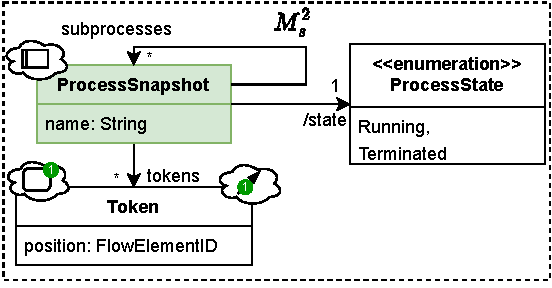
\includegraphics[width=0.475\textwidth]{figures/bpmn_s_model.pdf}
    \caption{BPMN snapshot metamodel $M_s^2$}
    \label{fig:bpmn_snapshot_model}
\end{figure}

\textsf{ProcessSnapshot}s are visualized using the concrete syntax of the underlying process.
In addition, \textsf{Token}s are highlighted with green bubbles in the middle of sequence flows or the top right of an activity.
The root of the \gls*{bpmn} snapshot metamodel is the \textsf{ProcessSnapshot}, highlighted in light green.

% Propositions need the global snapshot metamodel
Using the snapshot metamodels, one can only define atomic propositions for one model not spanning multiple models.
Thus, we must somehow merge all snapshot metamodels and the system relationship model into one model, describing a state/snapshot of the multi-model.
We call this model the \emph{global snapshot metamodel}.

% Merge description
To calculate the global snapshot metamodel, one must merge all snapshot metamodels with the system relationship model.
The first step is to add all model elements to one global model, i.e., calculating their disjoint\footnote{Possible conflicts due to the naming of model elements can be resolved by user input or a fixed strategy, for example, prefixing model elements with the model name.} union.

The second step is adding inheritance relations to connect behavioral models in the system relationship model with their corresponding snapshot metamodels.
Each behavioral model is typed in a behavioral metamodel, which has a snapshot metamodel structurally describing its state.
Thus, we know how the states of each behavioral model are structured by referring to its metamodel.
We make this knowledge explicit by adding an inheritance relation for each behavioral model to the root of the corresponding snapshot metamodel.
The resulting artifact, the \emph{global snapshot metamodel}, describes all possible states of the global system since each behavioral model inherits a description of its state.

% Merge example
\autoref{fig:global_execution_model} depicts the global snapshot metamodel $M_s^+$ for the use case, describing the states of the traffic management system.
We added three inheritance relations to construct $M_s^+$ for the use case and omitted unchanged parts from the system relationship model and the individual snapshot metamodels.

\begin{figure}[h]
    \centering
    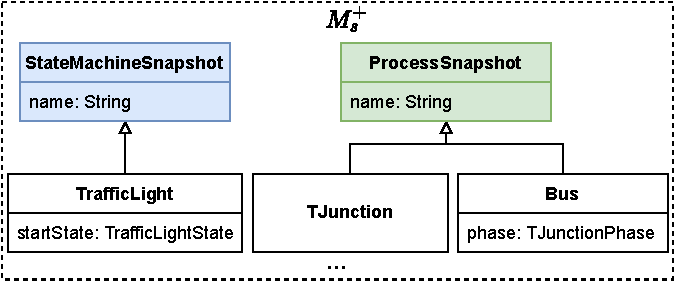
\includegraphics[width=0.475\textwidth]{figures/global_s_model.pdf}
    \caption{Global snapshot metamodel $M_s^+$ for the use case}
    \label{fig:global_execution_model}
\end{figure}

% Use case example propositions
Atomic propositions are formulated by providing an instance of $M_s^+$.
For example, \autoref{fig:atomic_propositions} shows how to formulate the atomic propositions $A_{green}$ and $B1_{passing}$, used in the global properties, stated earlier.
It is worth noting that the defined atomic propositions are \textit{special}, meaning they exactly fit the given multi-model and are not generally applicable to all state machines or \gls*{bpmn} models.

\begin{figure}[h]
    \centering
    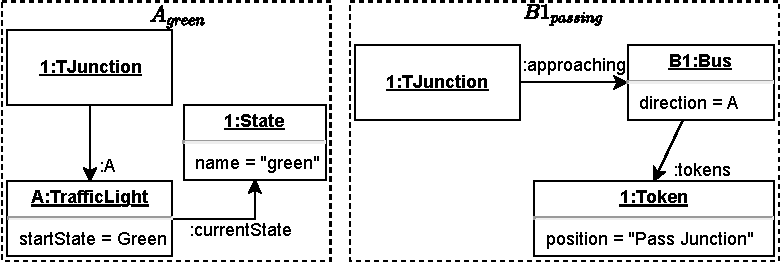
\includegraphics[width=0.475\textwidth]{figures/atomic_props.pdf}
    \caption{Atomic propositions $A_{green}$ and $B1_{passing}$}
    \label{fig:atomic_propositions}
\end{figure}

Alternatively, to make formulating atomic propositions less cumbersome, one can use the concrete syntax of the individual snapshot metamodels to formulate atomic propositions.
For example, \autoref{fig:atomic_propositions_concrete} shows the same atomic propositions as \autoref{fig:atomic_propositions} but uses the introduced concrete syntax.

\begin{figure}[h]
    \centering
    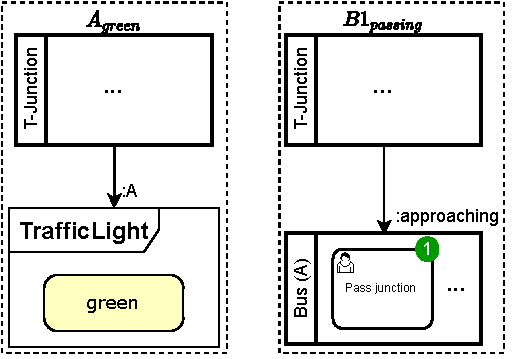
\includegraphics[width=0.4\textwidth]{figures/atomic_props_concrete.pdf}
    \caption{Concrete syntax for $A_{green}$ and $B1_{passing}$}
    \label{fig:atomic_propositions_concrete}
\end{figure}

Based upon the defined atomic propositions, one can then use temporal logic to define global behavioral properties such as the properties \ref{eq:property1}-\ref{eq:property4} in \autoref{sec:usecase}.

\subsection{Define model interactions}
Structural models in a multi-model might contain related information.
Thus, current approaches define so-called \emph{commonalities} to explicate these relationships and keep the information consistent \cite{stunkelComprehensiveSystemsFormal2021,klareCommonalitiesPreservingConsistency2019}.

To check the behavioral consistency of a system, we are primarily interested in global system behavior.
However, global behavior depends not only on the local behavior of the models, but also on their interactions.
Consequently, we call these inter-model relationships \emph{interactions} since they carry behavioral meaning while commonalities carry structural meaning \cite{krauterBehavioralConsistencyHeterogeneous2021}.

To specify interactions between different behavioral models, we defined an interaction language given by the interaction metamodel in \autoref{fig:interaction_metamodel}.
The interaction metamodel uses concepts from the system relationship metamodel (see \autoref{fig:systemRelationshipMetamodel}) since interactions can only be specified between behavioral models connected by \textsf{BehavioralRelationship}s.

In addition, we introduce the concept of \emph{state-changing elements}.
Each \textsf{BehavioralMetamodel} specifies a set of \textsf{StateChangingElement}s.
For example, a state machine defines states and transitions, but only the transitions describe how the states in a state machine change.
Thus, the transitions are the \textsf{StateChangingElement}s of a state machine (highlighted in purple, see \autoref{fig:fsm_metamodel}).
Similarly, the flow nodes are the \textsf{StateChangingElement}s of a \gls*{bpmn} process (highlighted in purple, see \autoref{fig:bpmn_metamodel})\footnote{One exception is the event-based gateway, which is not part of the \textsf{StateChangingElement}s.}.
The interaction of behavioral models is only possible through instances of the \textsf{StateChangingElement}s.

Our approach is based on the assumption that state-changing elements can be identified in metamodels for any behavioral formalism.
So far, we do not see any problems with this assumption since behavioral modeling languages must have some construct to describe state-change.
If we look at other popular examples, such as Petri Nets or \gls*{uml} activity diagrams, it is clear which constructs are the state-changing elements. 

\begin{figure}[h]
    \centering
    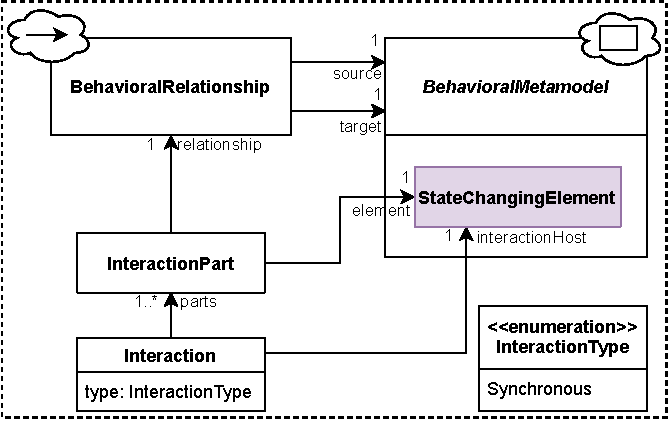
\includegraphics[width=0.475\textwidth]{figures/interaction_metamodel.pdf}
    \caption{Interaction metamodel}
    \label{fig:interaction_metamodel}
\end{figure}

An \textsf{Interaction} has an \textsf{interactionHost}, a set of interaction \textsf{parts} and an \textsf{InteractionType}.
Currently, there is only the \textsf{synchronous} \textsf{InteractionType}.
However, more interaction types, for example, asynchronous interactions or interactions with message passing, could be added in the future.
Asynchronous interactions can also be modeled using two synchronous interactions with an additional behavioral model, such as a queue.
Each \textsf{InteractionPart} references one \textsf{BehavioralRelationship} and one \textsf{StateChangingElement}.

The \textsf{interactionHost} and the elements of the \textsf{InteractionPart}s describe a state change for their concrete behavioral model.
By connecting them with a synchronous interaction, we define simultaneous state changes in one atomic step. 
Consequently, an interaction can define a synchronization between behavioral models.
In addition, each \textsf{InteractionPart} must be based on a \textsf{BehavioralRelationship} in the system relationship model, which must have the behavioral model containing the \textit{interactionHost} as a source and the behavioral model containing the \textsf{StateChangingElement} of the \textsf{InteractionPart} as a target.
Thus, one can only define interactions for behavioral models connected by behavioral relationships.

We allow the definition of as many interactions as desired.
The interactions restrict the local behavior of the models since some parts of their behavior must synchronize.
Two interactions sharing state changing elements is forbidden.
If such a situation occurs, it must be resolved by the modeler by deleting one of the interactions or merging the two interactions into one.

In the use case, the T-Junction controller interacts with the three traffic lights, \textbf{A}, \textbf{B}, and \textbf{C}.
\autoref{lst:interactions} defines two interactions synchronizing T-Junction controller and the traffic lights, using a textual \gls*{dsl}.
The \textbf{synchronize} keyword specifies the \textsf{InteractionType} to be \textsf{synchronous}.

\lstinputlisting[
label=lst:interactions,
language=Interaction,
caption=Interactions for the use case]{figures/interactions.txt}

We can explain the interactions as follows.
The first line defines that the interactions are specified from the viewpoint of the T-Junction in the system relationship model, i.e., \autoref{fig:systemRelationshipModel}.
The first interaction defines that the task \textsf{Switch to P1} and three other state changing elements synchronize.
Furthermore, line 3 specifies that one of the synchronization partners is the element \textit{turn green} connected by the relationship \textit{A}.
Similarly, two other transitions of the traffic lights \textit{B} and \textit{
C} are specified in the following two lines.
Thus, the interaction defines a synchronization of a task execution and three traffic light transitions. 
The second interaction defines a synchronization for the task \textsf{Switch to P2} and three other traffic light transitions.

\subsection{Check behavioral consistency}

By computing the global snapshot metamodel, we can represent the global states of the system, but we still need execution semantics to generate a state space to check the properties.
The execution semantics used in our approach must fulfill the following three requirements:
\begin{enumerate}
    \item The execution semantics must incorporate each behavioral model.
    \item The execution semantics must reflect the defined interactions between the behavioral models.
    \item The execution semantics must generate a state space, where each state can be interpreted as an instance of $M_s^+$, given a system configuration (instance of the system relationship model).
\end{enumerate}
Generally, our approach is independent of the underlying execution semantics if it fulfills the three requirements.
Thus, one can experiment with different underlying semantics, for example, graph transformations, rewriting logic, state machines, Petri nets, or process algebras, without changing the general framework.
One can then pick the most suitable semantics for the modeling scenario at hand regarding, for example, consistency checking performance.

To summarize, we obtain execution semantics, which describes the system's global behavior.
Generating these execution semantics from the models and interactions must be fully automated to allow frequent model changes.
However, execution semantics can be reused for all defined properties using varying atomic propositions. 
Later in the paper, we introduce execution semantics based on rewriting logic in Maude and apply them to the use case.
However, execution semantics based on graph transformations executable in the Groove tool set also exist. 

We can then use the constructed execution semantics for consistency checking by generating a state space based on a system configuration.
Since each state is an instance of $M_s^+$, we can interpret the constructed atomic propositions on the states.
An atomic proposition is true for a state if the corresponding instance of $M_s^+$ contains the atomic proposition.
Then, we can check consistency requirements on the generated state space.
This step should be fully automated, such that it can be executed as many times as needed (indicated by the loop in \autoref{fig:approach}) for different system configurations and consistency requirements (including atomic propositions) but using the same execution semantics.

Finally, if a consistency requirement is not fulfilled, a violation, including a counterexample based on the state space, should be presented to the user.
Adopting the same concrete syntax to visualize the counterexample as for the atomic propositions should be ideal for helping a user understand the counterexample easily. 
An unsuccessful consistency check leads to a consistency restoration process, which is crucial but out of scope for this contribution.
We describe consistency checking for the use case and its result in the end of the next section.
In addition, the appendix contains \autoref{fig:allConcepts}, which gives an overview of all the concepts introduced in this section and how they are applied to the use case.

\section{Global execution semantics} \label{sec:global_execution_semantics}
In this section, we will describe our implementations based on Groove\footnote{\url{https://groove.ewi.utwente.nl/about}} and Maude\footnote{\url{https://maude.cs.illinois.edu/w/index.php/The_Maude_System}}.
Then, we apply them to check behavioral consistency for the use case and discuss the results.

\subsection{Groove execution semantics} 
% TODO: Finalize this section.
% Missing:
% What is the type graph?

% Graph transformation rules and their generation from the behavioral models
This section describes one possible semantics to use in our approach to behavioral consistency management.
We will use graph transformation semantics based on graph grammars, see \autoref{def:graphGrammar}.

\begin{definition}[Graph grammar] \label{def:graphGrammar}
A graph grammar $GG=(S, P)$ consists of a start graph $S$ and a set of graph transformation rules $P$ \cite{ehrigFundamentalsAlgebraicGraph2006}. 
\end{definition}

The idea of a graph grammar is to begin with a start graph and then continuously apply all possible graph transformation rules.
Thus, one obtains a state space where each state is a graph, and each transition is a rule application.
Rules can be applied using different approaches, such as double-pushout (DPO) \cite{ehrigFundamentalsAlgebraicGraph2006} or single-pushout (SPO) \cite{loweAlgebraicApproachSinglepushout1993}.
Graph transformation rules for DPO are defined in \autoref{def:gtRule}.
Informally speaking, elements in $R$ but not in $L$ are added by a rule, while elements in $L$ and $R$ are preserved, and a rule deletes elements that are in $L$ but not in $R$.

\begin{definition}[Graph transformation rule] \label{def:gtRule}
A graph transformation rule $P= L \overset{l}{\leftarrow} K \overset{r}{\to} R$ consists of graphs L, K, R, and graph morphisms $l: K \to L$ and $r: K \to R$ \cite{ehrigFundamentalsAlgebraicGraph2006}. 
\end{definition}

The first step to generate global execution semantics is to generate a graph transformation rules for each behavioral model contained in the multi-model. % Relation from elements to rules needed!
Each set of rules must describe the behavior of the given behavioral model by manipulating instances of the snapshot metamodels.
For example, a graph transformation rule for a transition in a state machine changes the current state of a corresponding state machine snapshot from the source to the target state of the transition. 

Thus, we need a \emph{model transformation} to a set of graph transformation rules for each behavioral language.
Each model transformation only has to be implemented once by an \gls*{mde} tool developer and made available, for example, as a plugin, such that it can then be reused in any future setting the language is needed.
In addition, each model transformation must keep traces of the generated set of rules.
Concretely, it has to save which rules originated from which state-changing elements in the behavioral model.
Coming back to the state machine example, we must know which transition results in which graph transformation rule.
In general, multiple rules may be associated with one state-changing element of a behavioral model.
For example, a receive task in a \gls*{bpmn} process cannot be represented by only one rule, since it starts and then waits for an incoming message before finishing.

We apply the following steps to merge the obtained rules into rules describing the global execution semantics.
\begin{enumerate}
    \item All rules generated from state-changing elements not part of interactions remain unchanged and are added to the global rule set.
    \item For each interaction, we do the following:
     \begin{enumerate}
         \item Find the corresponding graph transformation rule\footnote{If one state-changing element results in more than one rule, one can define a strategy to pick the appropriate rule.
         For example, if one wants to synchronize with the start of a \gls*{bpmn} task, one can use a strategy to pick that rule.} $P_0$ for the interaction host of the interaction and find the rules $P_1, P_2, \ldots P_n$ for the state-changing elements taking part in the interaction using the saved traces.
         \item Calculate the parallel production \cite[Definition 3.2.7]{baldanConcurrentSemanticsAlgebraic1999} $P_0 + P_1 + \ldots + P_n$ for the found rules.
         Intuitively, applying a parallel production can be seen as applying multiple rules simultaneously, i.e., synchronizing the state changes of the behavioral models.
         \item For each part of the interaction, add a behavioral relationship from the behavioral model in $P_0$ to the behavioral model in $P_i$, for 0 < i $\leq$ n.
         The behavioral relationship is essentially a copy of the behavioral relationship referenced by that interaction part.
     \end{enumerate}
\end{enumerate}

As a type graph for the graph grammar, we utilize the global snapshot metamodel $M_s^+$ which fits rules coming from individual models and rules created by interactions.
Together with a system configuration, the set of typed global rules results in a graph grammar generating a state space.
Each state in this state space is an instance of the global snapshot metamodel.
Consequently, this can be used to check the behavioral consistency of the multi-model.

We will now explain how the graph transformation execution semantics are generated for the use case.
To apply our approach to the use case, we need to define model transformations from state machines and \gls*{bpmn} processes to graph transformation rules.

\subsubsection{State machine semantics}
The generation of graph transformation rules to implement finite state machine execution semantics is straightforward.
Each transition leads to a graph transformation rule.
For example, \autoref{fig:sm_rules} shows the graph transformation rules for the transitions \textsf{turn red-amber} and \textsf{turn green} of the traffic light model.
It uses the concrete syntax introduced in the paper to depict state machine snapshots and their current state.
We depict a graph transformation rule by showing its graph $L$ on the left, pointing with a named white arrow to its graph $R$ on the right.

\begin{figure}[h]
    \centering
    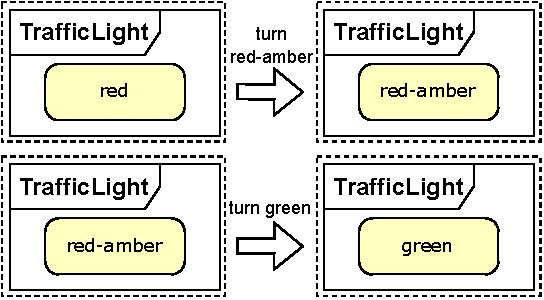
\includegraphics[width=0.425\textwidth]{figures/sm_rules.pdf}
    \caption{Graph transformation rules for \emph{turn red-amber} and \emph{turn green}}
    \label{fig:sm_rules}
\end{figure}

Using a traffic light snapshot with the state red as a start graph results in a graph grammar\footnote{\label{footnote:GGinRepo}All generated graph grammars, including further instructions regarding execution and consistency checking, can be found in \cite{krauterArtifactsBehavioralConsistency2022}.}, which will generate the same state space as the traffic light state machine.
We evaluated our approach by executing the graph grammar with the graph transformation tool Groove \cite{ghamarianModellingAnalysisUsing2012, rensinkGROOVESimulatorTool2004}.
However, in the future, we can also experiment with other graph transformation tools since rule generation can be adapted without much effort.
% Programming against a clearly defined interface makes this possible. But that's not important for this paper.

\subsubsection{BPMN semantics}
The generation of graph transformation rules for \gls*{bpmn} processes is challenging, and we are currently only supporting a subset of the \gls*{bpmn} semantics, similar to the extent supported by \cite{vangorpVisualTokenbasedFormalization2013}.
Generally, we construct one or more rules for each flow node contained in a \gls*{bpmn} process.
\autoref{fig:bpmn_example_rules} shows graph transformation rules for some flow nodes of the T-Junction controller.
It uses the concrete syntax introduced earlier to represent process snapshots containing tokens.

\begin{figure}[h]
    \centering
    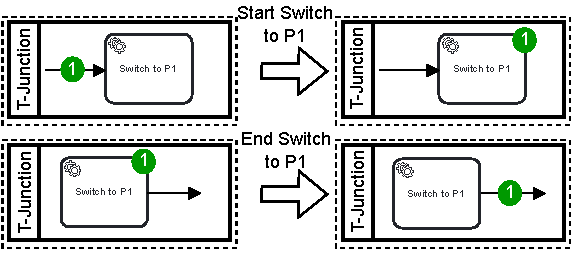
\includegraphics[width=0.475\textwidth]{figures/bpmn_rules.pdf}
    \caption{Example graph transformation rules for the T-Junction controller}
    \label{fig:bpmn_example_rules}
\end{figure}

However, we cannot show all possible rules resulting from our \gls*{bpmn} semantics implementation.
Especially the implementation of signal events, message events, event-based gateways, and subprocesses needs further explanation but does not matter for the overall approach presented in this paper, as long as it conforms to the \gls*{bpmn} semantics.
We compared the state space resulting from our implementation with the possible token flows realizable using the \emph{bpmn-js token simulation}\cref{footnote:GGinRepo}, which claims to conform to the \gls*{bpmn} semantics.
This resulted in finding bugs in the bpmn-js simulator and our rule generator.

Our semantics is inspired by \cite{vangorpVisualTokenbasedFormalization2013} but differs in some aspects.
One key difference is that they define a fixed rule set that describes the semantics of \gls*{bpmn} models, while we generate a specific rule set for each model to enable interaction with specific parts of each model.
The rule generation is implemented in Java and can be found in \cite{krauterRewriteRuleGeneration2022}.

Following this procedure, we can generate graph transformation rules that implement the behavioral semantics of the \gls*{bpmn} models in the use case\cref{footnote:GGinRepo}.

\subsubsection{Check behavioral consistency}
The defined interactions change the rules for switching to phases 1 and 2.
\autoref{fig:parallel_rule} shows the resulting rule for switching to phase 1.
We decided that the interactions between the traffic lights and the T-Junction controller should synchronize with the end of the task, not the start.

\begin{figure}[h]
    \centering
    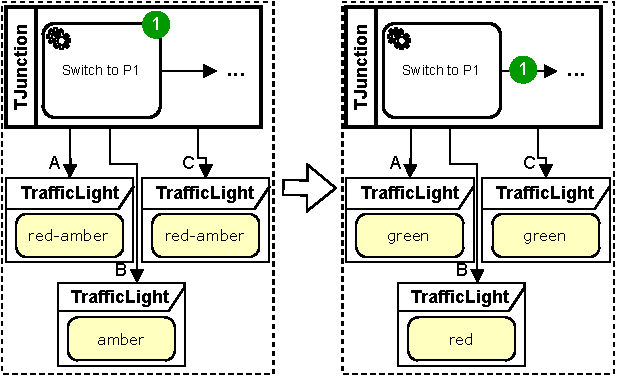
\includegraphics[width=0.475\textwidth]{figures/parallel_rule.pdf}
    \caption{Global graph transformation rule to switch to phase 1}
    \label{fig:parallel_rule}
\end{figure}

The rule changes all traffic lights simultaneously and finishes the task.
The corresponding individual rules no longer exist, so synchronization of the behavior is guaranteed.
A similar rule exists for switching to phase 2, resulting from the other interaction.
All other rules are left untouched during the construction of the global graph grammar.

Finally, we can generate the global state space of the system using the global graph grammar\cref{footnote:GGinRepo}.
To check the requirements formalized by properties 1-4, we must ensure the generated state space contains the needed atomic propositions.
All atomic propositions are specified as instances of $M_s^+$ that can be converted to graph conditions in Groove.
Graph conditions in Groove are rules that do not change elements but can be used as atomic propositions in model checking.

\subsection{Maude execution semantics}
We are using the predefined Maude module for object-based programming to encode the snapshot metamodels in Maude.
In addition, we add behavioral relationships from the interaction metamodel, such that we can instantiate them to create the system configuration described in the use case.

Interactions lead to rule merges in Maude where the left and right side of each individual rule is added to a global rules.
Furthermore, behavioral relationships as defined in the interaction are added to the rule.
Similarly to the process for graph transformation rules, individual rules are deleted.

\subsubsection{State machine semantics}

We are using the predefined Maude module for object-based programming to encode the state machine snapshot metamodel in Maude.
This encoding has to be only done once, similar to the type graph definition in Groove.

The generation of rewriting rules is similar to the generation of graph transformation rules.
Each state machine transition leads to one rewriting rule.
\autoref{lst:trafficLightMaude} shows the rewriting rules for the traffic light model.
In addition, based on the defined start state, a start configuration is generated (see lines 7 and 8).
The start configuration is the Maude counterpart of the start graph in graph grammars.

\lstinputlisting[
label=lst:trafficLightMaude,
language=Interaction,
float=*,
caption=Rewriting rules and start configuration for a traffic light]{figures/trafficLight.maude}

Using Maude's search command and search graph visualization, we can verify that the generated state space conforms to the traffic light state machine\footnote{\label{footnote:maudeArtifacts}The corresponding Maude files and example Maude executions can be found in \cite{krauterArtifactsBehavioralConsistency2022}}.

\subsubsection{BPMN semantics}
Again we encode the \gls*{bpmn} snapshot metamodel in Maude using the predefined module for object-based programming.
The rewriting rule generation is similar to the graph transformation rule generation and supports the same subset of \gls*{bpmn} semantics.
Similarly, one or more rules are constructed for each flow node in a \gls*{bpmn} process.
\autoref{lst:tJunctionControllerMaude} shows two Maude rewriting rules for the first two flow nodes of the T-Junction controller as depicted in \autoref{fig:bpmn_example_rules}.
The remaining rules can be found in \cite{krauterArtifactsBehavioralConsistency2022}.

\lstinputlisting[
label=lst:tJunctionControllerMaude,
language=Interaction,
float=*,
caption=Example rewriting rules for the T-Junction controller]{figures/tJunctionController.maude}

Like the graph transformation rules, the rewriting rules move tokens by changing their position according to the given \gls*{bpmn} model.
Thus, we can generate rewriting rules that implement the behavioral semantics of the \gls*{bpmn} models in the use case.
The rule generation is implemented in Java and can be found in \cite{krauterRewriteRuleGeneration2022}.

\subsubsection{Check behavioral consistency}
The defined interactions change the rules for switching to phases 1 and 2. \autoref{lst:synchRuleMaude} shows the resulting rule for switching to phase 1, where a synchronization with the end of the task was chosen.
\autoref{fig:parallel_rule} shows the equivalent graph transformation rule.

\lstinputlisting[
label=lst:synchRuleMaude,
language=Interaction,
float=*,
caption=Global Maude rule to switch to phase 1]{figures/synch.maude}

The rule changes all traffic lights simultaneously and finishes the task.
Similarly, a global rule for switching to phase 2 is created and all individual rules are deleted.

Finally, we can use the Maude model checker module to check the requirements formalized by the \gls*{ltl} properties 1-4\cref{footnote:maudeArtifacts}.
Atomic propositions can be represented in Maude using the encoded snapshot metamodels and behavioral relationships.

\subsection{Behavioral consistency in the use case}

Both implementations show that properties 1 and 2 hold, while properties 3 and 4 do not hold\cref{footnote:GGinRepo}\cref{footnote:maudeArtifacts}.
The counterexamples for properties 3 and 4 show an unexpected race condition that must be handled.
After the T-Junction controller signals that the traffic light A/B is green, bus B1/B2 can advance to the \textsf{Pass Junction} activity.
However, at the same time, the T-Junction controller can enter the subprocess for the next phase, which can be interrupted by the associated timer event.
This can happen before the bus B1/B2 passes the junction, resulting in an invalid state.

The system developers have different options to handle the uncovered inconsistencies.
One option is to keep the models unchanged and pay special attention to the found race condition during system implementation.
This can be an acceptable solution since the \textsf{Pass Junction} activity is also modeled as a user activity, i.e., the bus driver decides when to cross the T-Junction.
Furthermore, tolerating inconsistencies can be a viable option in \gls*{mde} \cite{weidmannToleranceModelDrivenEngineering2021}.
Another option is to change the models to resolve the inconsistency.
For example, the T-Junction controller could wait for the bus to pass before changing the traffic lights again.

\section{Related work} \label{sec:related_work}
This contribution builds on our previous publication \cite{krauterBehavioralConsistencyHeterogeneous2021}.
However, we refined the behavioral consistency management workflow by introducing new concepts such as the system relationship model and snapshot metamodel.
Moreover, we created an interaction language and outlined a general approach to define atomic propositions, leading to global behavioral properties.
In addition, our previous work did not support \gls*{bpmn} models.

% Highlight some specific combinations/ad-hoc approaches for a single modeling language.
The general idea of transforming different behavioral formalisms to a single semantics domain to reason about cross-cutting concerns is not new, see, e.g. \cite{engelsMethodologySpecifyingAnalyzing2001}.
For example, \cite{kusterExplicitBehavioralConsistency2003} developed consistency checking for sequence diagrams and statecharts based on \gls*{csp}, while \cite{yaoConsistencyCheckingUML2006} used Petri nets for the same scenario.
Furthermore, \cite{cunhaFormalVerificationUML2011} analyze sequence diagrams in the context of embedded systems using a transformation to Petri nets.
Nevertheless, all approaches focus on a single modeling language or a fixed combination of two languages.
Consequently, they do not consider the general problem of behavioral consistency in a heterogeneous modeling scenario.

% Kienzle with event structures
\cite{kienzleUnifyingFrameworkHomogeneous2019} proposes a unifying framework for homogeneous model composition.
To combine behavioral models, they use Event structures \cite{winskelEventStructures1987} as an underlying formalism and show how different homogeneous behavioral models can be combined.
Nonetheless, they do not apply their approach to heterogeneous models.
Generally, their approach is compatible with ours since we do not mandate a specific formalism in our approach.
However, we have chosen graph transformation rules as the first formalism to use in our approach since they operate on a higher abstraction level.
In addition, it was shown that many formalisms, for example, the $\pi$-calculus \cite{gadducciGraphRewritingPcalculus2007}, can be implemented using graph transformation rules.

% Gemoc Studio/BCOOL?
% Approach is quite technical (i.e., execution engine. No formal execution semantics?)
\cite{deantoniModelingBehavioralSemantics2016} tackles the problem of dealing with relationships between heterogeneous behavioral models.
They coordinate the different models using their coordination language B-COoL \cite{varalarsenBCoolBehavioralCoordination2016}, similar to the interactions we define between behavioral models.
To execute the models and their coordination, they transform them into \gls*{ccsl} models.  
Their work also results in plugins for GEMOC studio, which support running and debugging the models.
% Ptolemy
\cite{ekerTamingHeterogeneityPtolemy2003, leeDisciplinedHeterogeneousModeling2010} propose an actor-oriented solution to the model composition problem in the presence of heterogeneity.
Their approach results in the tool Ptolemy \cite{ptolemaeusSystemDesignModeling2014}.

% very nice, but only simulation for Ptolemy and no real verification support (LTL model checking and atomic prop definition) in BCool/Gemoc.
However, both approaches focus on simulation rather than consistency or model-checking.
Neither provides concrete means to define atomic propositions and check global behavioral properties.

\section{State space explosion} \label{sec:state_space_explosion}
State space explosion is one of the predominant issues when applying model checking to complex systems, as they are often found in real-world applications.
As one can see in \autoref{table:maudeRuntime} and \autoref{table:grooveRuntime} our approach is not immune to state space explosion.
The tables show the states, rewrites/transitions, and average runtime of a full state space exploration in the Maude and Groove-based implementations.
Four scenarios were benchmarked, starting with the use case multi-model without approaching buses and then increasing the number of buses up to three.

To calculate the average runtime, we used the hyperfine benchmarking tool \cite{peterHyperfine2022} (version 1.15.0), which ran state space exploration for each scenario ten times.
Timing evaluations were done on a notebook with an AMD Ryzen PRO 3500U processor and 16 GB of RAM running Maude version 3.2.1 (inside the Windows Subsystem for Linux) and Groove version 5.8.1.

The benchmarks include start-up times, for example, the state space exploration for the \textsf{No Buses} scenario takes \textasciitilde 500ms according to Groove.
Thus, most of the exploration time in Maude and Groove for the \textsf{No Buses} scenario is attributed to the start-up time.
Generally, the Maude exploration time is lower despite larger state spaces due to technical differences in implementing the \gls*{bpmn} semantics.
However, as expected, neither of the tools is immune to state space explosion.

\begin{table}
\centering
\begin{tabular}{|c || c | c | c |}
 \hline
 Use case & States & Rewrites & Exploration time \\
 \hline\hline
 No buses & 168 & 664 & \textasciitilde 63.3 ms \\
 \hline
 1 bus & 3.304 & 19.958 & \textasciitilde 277.8 ms \\
 \hline
 2 buses & 35.280 & 27.9776 & \textasciitilde 2.994 ms \\
 \hline
 3 buses & 260.176 & 2.522.582 & \textasciitilde 28.091 ms \\
 \hline
\end{tabular}
\caption[State space exploration in Maude]{State space exploration in Maude\footnotemark}
\label{table:maudeRuntime}

\bigskip

\begin{tabular}{|c || c | c | c |}
 \hline
 Use case & States & Transitions & Exploration time \\
 \hline\hline
 No buses & 168 & 438 & \textasciitilde 2.948 ms \\
 \hline
 1 bus & 2.888 & 10.046 & \textasciitilde 4.510 ms \\
 \hline
 2 buses & 27.880 & 121.554 & \textasciitilde 11.629 ms \\
 \hline
 3 buses & 195.336 & 1.028.340 & \textasciitilde 63.487 ms \\
 \hline
\end{tabular}
\caption[State space exploration in Groove]{State space exploration in Groove\cref{footnote:benchmark}}
\label{table:grooveRuntime}

\end{table}

\footnotetext{\label{footnote:benchmark}A description how to run the benchmarks can be found in \cite{krauterArtifactsBehavioralConsistency2022}.}

% Discussion
% Full state space is not what you do. You check properties.
As in our use case, one is generally not interested in a full state space exploration as in \autoref{table:maudeRuntime} and \autoref{table:grooveRuntime} but rather in the validity of a set of behavioral properties.
Checking, for example, a property specified in \gls*{ltl}, does not necessarily lead to a full state space exploration.
Furthermore, not every property is concerned with all behavioral models.
For example, properties (1) and (2) of the use case do not involve buses and can be checked on the much smaller state spaces, not including approaching buses.
In addition, checking a set of properties can be run in parallel.
If some properties show to be computationally expensive, they can be run on dedicated hardware, for example, during a continuous integration pipeline once a day in case of behavioral model or interaction changes.
Thus, checking the consistency of a multi-model can be seen as an additional test during \gls*{mde}, which can be run locally but, in addition, is a vital part of continuous integration.

% Ways to mitigate state space explosion.
The Maude \gls*{ltl} model-checker has performance comparable to the popular SPIN model checker \cite{ekerMaudeLTLModel2004} and thus is proven to have a good performance.
However, one could use different techniques to mitigate the state space explosion problem further.
One technique is to abstract models further such that they only contain information relevant to the set of properties to be checked.
Thus, minimal models are synchronized, leading to smaller state spaces.
However, finding correct minimal models might not be trivial.

Partial-order reduction is a well-known and successful technique to mitigate the state space explosion problem.
It is currently not implemented in the Maude LTL model-checker, but there is promising work to integrate partial-order reduction into the model-checker \cite{farzanPartialOrderReduction2007}, showing substantial state space reductions.
The potential to reduce the state space using this technique is huge, especially for model-checking concurrent systems \cite{clarkeHandbookModelChecking2018}.
Our approach analyzes concurrent systems with some interaction, and thus model-checking would greatly benefit from partial-order reduction.
Partial-order reduction is most likely a must to analyze models from real-world applications.

\section{Conclusion and future work} \label{sec:conclusion_and_future_work}
% Conclusion
Our work represents the first general fully-formalized approach to behavioral consistency management in a heterogeneous modeling scenario, enabling formulating and checking \emph{global} properties.
Previous work either only dealt with the behavioral consistency between specific pairs of models \cite{yaoConsistencyCheckingUML2006, kusterExplicitBehavioralConsistency2003} or focused on the simulation in a heterogeneous scenario \cite{deantoniModelingBehavioralSemantics2016, varalarsenBCoolBehavioralCoordination2016, ekerTamingHeterogeneityPtolemy2003, leeDisciplinedHeterogeneousModeling2010}.

Our approach follows three key steps (see \autoref{fig:approach}).
% Describe the three steps
First, we align the behavioral models by defining their interactions.
Then, we generate global execution semantics based on the defined interactions while preserving the original behavior of the models.
Finally, we can check the global consistency of the system in different configurations with varying consistency requirements using the generated semantics.
In addition, simulation of the multi-model and its interactions based on the user choosing the available actions is possible.
Although our approach is independent of a particular formalism as an underlying global execution semantics, the
current two implementations utilize rewriting logic (Maude) or graph transformations (Groove).

In future work, extending the execution semantics to include other behavioral formalisms such as activity diagrams, hierarchical state machines, and the $\pi$-calculus is interesting.
Especially integrating the $\pi$-calculus, which was formalized using graph grammars in \cite{gadducciGraphRewritingPcalculus2007}, will be beneficial since it is profoundly different from the currently supported formalisms.

% Data transfer
Furthermore, two systems often exchange data while interacting, for example, using messaging.
The exchanged data then greatly influences the future behavior of the systems.
Thus, adding data transfers to interactions between heterogeneous models is an important issue left for future work.

% Runtime verification
Finally, it is important to check that running systems are behaving as specified in their behavioral models, including the defined interactions between them.
Thus, extending runtime verification techniques to include systems specified by a multi-model with interactions constitutes a challenging problem.
% Could write about continuous time models to be included in the future.

\bibliography{bib}
\section*{About the authors}

\shortbio{Tim Kräuter}{is a Ph.D. research fellow at the Western Norway University of Applied Sciences, Bergen, Norway.
His primary research is on integrating heterogeneous behavioral models in multi-model-driven software engineering.
Previously he worked as a software developer at SET GmbH in Germany and acquired a master of science in Information Engineering at the University of Applied Sciences, FHDW Hannover, Germany.
\authorcontact[https://timkraeuter.com/]{tkra@hvl.no}}

\shortbio{Harald König}{is a professor for Computer Science at the University of Applied Sciences, FHDW Hannover, Germany, and an Adjunct Professor at the Department of Computer Science, Electrical Engineering and Mathematical Sciences at the Western Norway University of Applied Sciences, Bergen, Norway.
Before entering academia, he worked at SAP in Walldorf and received his Ph.D. in pure Mathematics from Leibniz University in Hannover, Germany. \authorcontact{harald.koenig@fhdw.de}}

\shortbio{Adrian Rutle}{is a professor at the Department of Computer science, Electrical engineering and Mathematical sciences at the Western Norway University of Applied Sciences, Bergen, Norway.
Rutle’s main interest is applying theoretical results from the field of model-driven software engineering to practical domains and has his main expertise in the development of formal modeling frameworks for domain-specific modeling languages, graph-based logic for reasoning about static and dynamic properties of models, and the use of model transformations for the definition of the semantics of modeling languages.
His recent research focuses on multilevel modeling, model repair, multi-model consistency management, modeling and simulation for robotics, digital fabrication, smart systems, and applications of machine learning in model-driven software engineering.
\authorcontact{aru@hvl.no}}

\shortbio{Yngve Lamo}{is a professor at the Department of Computer science, Electrical engineering and Mathematical sciences at the Western Norway University of Applied Sciences, Bergen.
Lamo holds a Ph.D. in Computer Science from the University of Bergen, Norway. His research interests span from formal foundations of Model Based Software Engineering to its applications, especially in Health Informatics.
He is currently applying MDSE to create Adaptive Software Technologies for mental Health. \authorcontact{yla@hvl.no}}

\shortbio{Patrick Stünkel}{is currently working as a postdoctoral researcher at Haukeland University Hospital in Bergen, Norway, where he is working on applying process mining, workflow modeling, and optimization techniques in digital pathology.
Before that, Patrick did his Ph.D. at Western Norway University of Applied Sciences on the topics of semantic interoperability and consistency management among heterogeneous software models.
\authorcontact[https://past.corrlang.io/]{Patrick.Stunkel@helse-bergen.no}}

\begin{figure*}[ht]
    \centering
    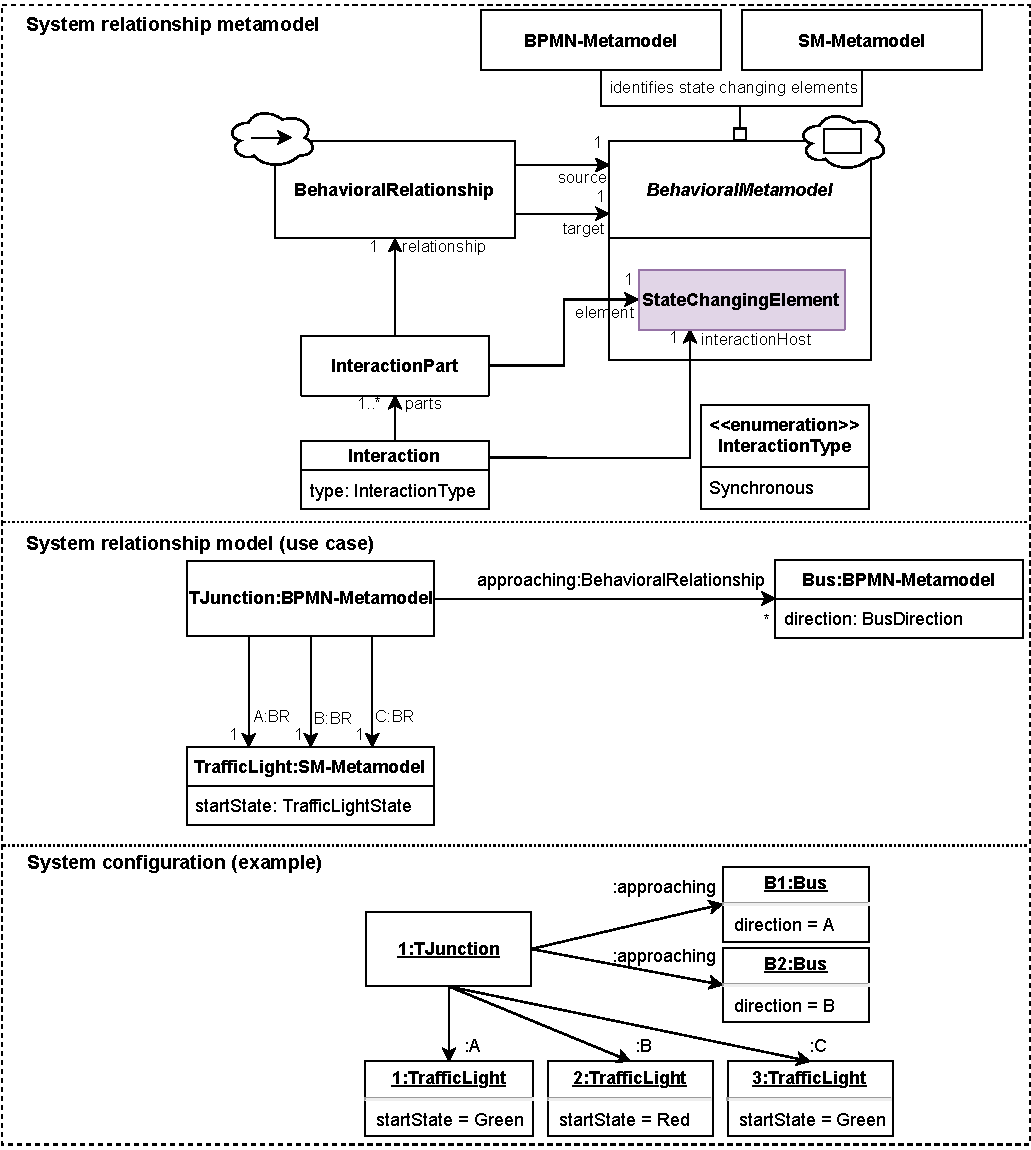
\includegraphics[width=1\textwidth]{figures/allConcepts.pdf}
    \caption{Overview of all concepts and their usage in the use case}
    \label{fig:allConcepts}
\end{figure*}

\end{document}